\documentclass[12pt,a4paper,oneside]{book}

\usepackage[left=2.54cm, right=2.54cm, top=2.54cm, bottom=2.54cm]{geometry}

% fonts packages 

\usepackage{float}
\usepackage[utf8]{inputenc}
\usepackage[T1]{fontenc}
\usepackage[spanish,es-noshorthands]{babel}

%Mathematical packages

\usepackage{amsfonts,amsmath,bussproofs,tabstackengine,amsthm}

% Graphical packages

\usepackage{graphicx}
\usepackage{tikz}
\usepackage{array} 
\usepackage{subcaption}
\usepackage{enumitem}
\usepackage{cancel}

% Index and bibliography packages

\usepackage{csquotes}
\usepackage[hidelinks]{hyperref}
\usepackage[backend=biber,style=apa]{biblatex}
\usepackage{amsmath, amssymb, graphics, setspace}


% Personal configurations

\addbibresource{research3.bib}
\newcommand{\diff}{\mathrm{d}}
\usetikzlibrary{arrows.meta,arrows}
\newcommand{\mathsym}[1]{{}}
\newcommand{\unicode}[1]{{}}
\renewcommand{\baselinestretch}{2}
\renewcommand{\qedsymbol}{$\blacksquare$}
\DeclareMathOperator{\sech}{sech}
\DeclareMathOperator{\csch}{csch}
\DeclareMathOperator{\arcsec}{arcsec}
\newtheorem{theorem}{Teorema}
\newtheorem{lemma}{Lema}
\newtheorem{proposition}{Proposición}
\newtheorem{corollary}{Corolario}
\newtheorem{definition}{Definición}

% Article information 

\author{Daniel Alejandro Reinoso Salas\\ César Daniel Reinoso Reinoso}
\begin{document}
\begin{titlepage}
    \thispagestyle{empty}
    \begin{minipage}[c][0.17\textheight][c]{0.25\textwidth}
        \begin{center}
            
\includegraphics[width=3.5cm, height=3.5cm]{images.jpg}
        \end{center}
    \end{minipage}
    \begin{minipage}[c][0.195\textheight][t]{0.75\textwidth}
        \begin{center}
            \vspace{0.3cm}
            \textsc{\large ESCUELA SUPERIOR POLITÉCNICA DE CHIMBORAZO}\\[0.5cm]
            \vspace{0.3cm}
            \hrule height2.5pt
            \vspace{.2cm}
            \hrule height1pt
            \vspace{.8cm}
            \textsc{FACULTAD DE CIENCIAS\\
                CARRERA DE MATEMÁTICAS }\\[0.5cm] %
        \end{center}
    \end{minipage}

    \begin{minipage}[c][0.81\textheight][t]{0.25\textwidth}
        \vspace*{5mm}
        \begin{center}
            \hskip2.0mm
            \vrule width1pt height13cm
            \vspace{5mm}
            \hskip2pt
            \vrule width2.5pt height13cm
            \hskip2mm
            \vrule width1pt height13cm \\
            \vspace{5mm}
            
\includegraphics[height=4.0cm]{logo-blanco (1).png}
        \end{center}
    \end{minipage}
    \begin{minipage}[c][0.81\textheight][t]{0.75\textwidth}
        \begin{center}
            \vspace{1cm}

            {\large\scshape Cuadricas}\\[.2in]
            \vspace{2cm}
            \textsc{\large Investigacion Formativa}\\[0.5cm]
            \textsc{\large Presenta:}\\[0.5cm]
            \textsc{\large {Daniel Alejandro Reinoso Salas \\
                    César Daniel Reinoso Reinoso\\
                    Fernando Gualpa Villasis}}\\[2cm]

            \vspace{0.5cm}

             {\large\scshape Tutor:\\[0.3cm] {Dra.   Zoraida Sivoli Barrios }}\\[.2in]

            \vspace{0.5cm}

            \large{Ecuador-Riobamba }{2022}
        \end{center}
    \end{minipage}
\end{titlepage}
\tableofcontents
\listoffigures
\newpage
\chapter{Introducción}
\chapter{Cuádricas}
\section{Definición}
Nos interesan las superficies de ecuación $z=f(x, y)$ o $F(x, y, z)=0$, es decir, las superficies formadas por los puntos $(x, y, z)$ que satisfacen la ecuación $z=f(x, y) \circ F(x, y, z)=0$.

En particular trabajaremos únicamente con superficies cuádricas cuyas ecuaciones están dadas en forma canónica.

Existen seis tipos básicos de superficies cuádricas: Elipsoide, Hiperboloide de una hoja, Hiperboloide de dos hojas, Cono Elíptico, Paraboloide Elíptico y Paraboloide Hiperbólico. \cite{solis2016graficas}.
\subsection{Elipsoide}
Ecuación canónica:
$$
    \frac{(x-i)^{2}}{a^{2}}+\frac{(y-j)^{2}}{b^{2}}+\frac{(z-k)^{2}}{c^{2}}=1
$$
Parametrización:
$$
    s(u, v):\left\{\begin{array}{l}
        x=i-a \cos u \operatorname{sen} v                 \\
        y=j-b \operatorname{sen} u \operatorname{sen} v ; \\
        z=k-c \cos v
    \end{array} \quad u \in[0,2 \pi], v \in[0, \pi]\right.
$$

\subsection{Hiperboloide de una hoja}
Ecuación canónica:
$$
    \frac{(x-i)^{2}}{a^{2}}+\frac{(y-j)^{2}}{b^{2}}-\frac{(z-k)^{2}}{c^{2}}=1
$$
Parametrización:
$$
    s(u, v):\left\{\begin{array}{l}
        x=i-a \cos u \cosh v                 \\
        y=j-b \operatorname{sen} u \cosh v ; \\
        z=k-c \operatorname{senh} v
    \end{array} \quad u \in[0,2 \pi], v \in \mathbb{R}\right.
$$

\subsection{Hiperboloide de dos hoja}
Ecuación canónica:
$$
    -\frac{(x-i)^{2}}{a^{2}}-\frac{(y-j)^{2}}{b^{2}}+\frac{(z-k)^{2}}{c^{2}}=1
$$
Parametrización:
$$
    s(u, v):\left\{\begin{array}{l}
        x=i+a \senh u \cos v                 \\
        y=j+b \operatorname{senh} u \sen v ; \\
        z=k+c \operatorname{cosh} u
    \end{array} \quad u \in[0, + \infty], v  \in[0,2 \pi] \right.
$$

\subsection{Cono elíptico centrado}
Ecuación canónica:
$$
    \frac{(x-i)^{2}}{a^{2}}+\frac{(y-j)^{2}}{b^{2}}-\frac{(z-k)^{2}}{c^{2}}=0
$$
Parametrización:
$$
    s(u, v):\left\{\begin{array}{l}
        x=i+\frac{a}{c} \operatorname{senh} u \cos v                 \\
        y=j+\frac{b}{c} \operatorname{senh} u \operatorname{sen} v ; \\
        z=k+\operatorname{senh} u
    \end{array} \quad u \in \mathbb{R}, v \in[0,2 \pi]\right.
$$

\subsection{Paraboloide elíptico}
Ecuación canónica:
$$
    z-k=\frac{(x-i)^{2}}{a^{2}}+\frac{(y-j)^{2}}{b^{2}}
$$
Parametrización:
$$
    s(u, v):\left\{\begin{array}{l}
        x=u \\
        y=v \\
        z=\frac{(u-i)^{2}}{a^{2}}+\frac{(v-j)^{2}}{b^{2}}+k
    \end{array} ; \quad u \in \mathbb{R}, v \in \mathbb{R}\right.
$$

\subsection{Paraboloide Hiperbólico}
Ecuación canónica:
$$
    z-k=-\frac{(x-i)^{2}}{a^{2}}+\frac{(y-j)^{2}}{b^{2}}
$$
Parametrización:
$$
    s(u, v):\left\{\begin{array}{l}
        x=u \\
        y=v \\
        z=-\frac{(u-i)^{2}}{a^{2}}+\frac{(v-j)^{2}}{b^{2}}+k
    \end{array} ; \quad u \in \mathbb{R}, v \in \mathbb{R}\right.
$$
\subsection{Ejemplo}

Considere el elipsoide y el hiperboloide de ecuación:
$$
    \frac{(x-1)^{2}}{4}+\frac{(y-3)^{2}}{1}+\frac{(z-1)^{2}}{9}=1
$$
y

$$
    \frac{(x+1)^{2}}{1}+\frac{y^{2}}{4}-\frac{(z-1)^{2}}{9}=1
$$
Encontrar el centro de las figuras.

\begin{figure}[H]
    \centering
    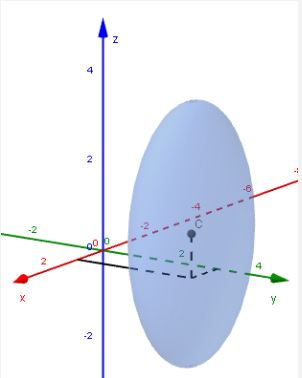
\includegraphics[width=6cm]{imagenes/Captura.jpg}
    \caption{Gráficas utilizando Geogebra para Elipsoide}
\end{figure}

\begin{figure}[hbtp]
    \centering
    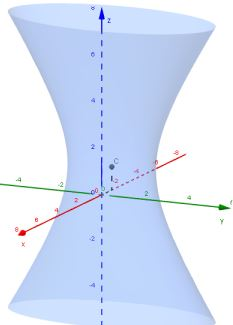
\includegraphics[width=6cm]{imagenes/Captura2.jpg}
    \caption{Gráficas utilizando Geogebra para Hiperboloide}
\end{figure}

\begin{tabular}{|c|c|c|c|}
    \hline
                 & Centrada en x & Centrada en y & Centrada en Z \\
    \hline
    Elipsoide    & 1             & 3             & 1             \\
    \hline
    Hiperboloide & -1            & 0             & 1             \\
    \hline
\end{tabular}

\chapter{Funciones de dos variables}
En estudios anteriores, hemos revisado funciones de una variable $f: \mathbb{R} \rightarrow \mathbb{R}$,
en esta sección revisaremos funciones de dos variables es decir, $f: \mathbb{R}^{2} \rightarrow \mathbb{R}$,
las funciones dos variables permiten el estudio de la densidad de la tierra, la presión de un globo, ciertos modelos matemáticos están descritos por funciones de dos variables.\par
\section{Definición}
Recuperado de \cite{strang}.\par
Una función de dos variables $z=f(x, y)$ mapea cada par ordenado $(x, y)$ en un subconjunto $D$ del plano real $\mathbb{R}^{2}$ a un único número real $z$. El conjunto $D$ se llama dominio de la función. El rango de $f$ es el conjunto de todos los números reales $z$ que tiene al menos un par ordenado $(x, y) \in D$ tal que $f(x, y)=z$ como se muestra en la siguiente figura.\par
\begin{figure}[H]
    \centering
    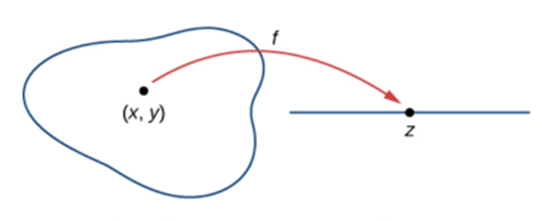
\includegraphics[width=9.5cm, height=5.5cm]{imagenes/NImagen1.png}
    \caption{El dominio de una función de dos variables consta de pares ordenados $(x, y)$.}
\end{figure}
\textbf{Nota:} Si una función $z=f(x, y)$ viene dada por una fórmula, asumimos que su dominio consta de todos los puntos $(x, y)$ para los cuales la fórmula tiene sentido, a menos que se especifique un dominio diferente.\par
\subsection{Gráfica de una función de dos variables}
La grafica de una función de dos variables es el conjunto de puntos $(\mathrm{x}, \mathrm{y}, \mathrm{z})$ tales que $z=f(x, y) y \quad x \in D$. Es decir,\par
$$
    \operatorname{Graf}(f)=\{(x, y, f(x, y)) \mid(x, y) \in D\}
$$
Tal que su representación seria.\par
\begin{figure}[H]
    \centering
    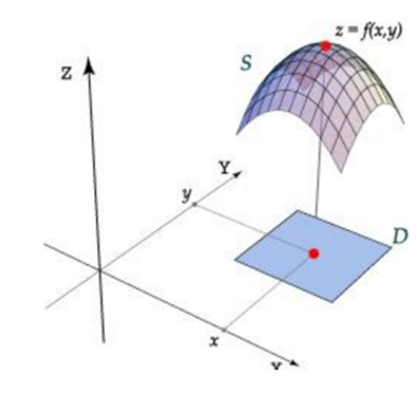
\includegraphics[width=9.5cm, height=7.5cm]{imagenes/Imagen4.png}
    \caption{Función de dos variables.}
\end{figure}
\newpage
\subsection{Ejemplo}

Representaciones geométricas de una tabla.\par
Recuperado de \cite{strang}, Suponga que la función $f$ está representada por la siguiente tabla:\par
\begin{table}[H]
    \centering
    \caption{Tabla de dos Entradas}
    \begin{tabular}{|c|c|c|c|c|}
        \hline                & $y=0$ & $y=1$ & $y=2$ & $y=3$ \\
        \cline { 2 - 5 }$x=0$ & 0     & 5     & 10    & 15    \\
        \cline { 2 - 5 }$x=1$ & 10    & 15    & 20    & 25    \\
        \hline$x=2$           & 20    & 25    & 30    & 35    \\
        \hline$x=3$           & 30    & 35    & 40    & 45    \\
        \hline
    \end{tabular}
    \bigskip
\end{table}

Geométricamente, podemos ver la información contenida en la tabla colocando primero un punto para cada $(x, y)$ en la tabla en el plano $x y$ de nuestro 3 -espacio\par

\begin{figure}[H]
    \centering
    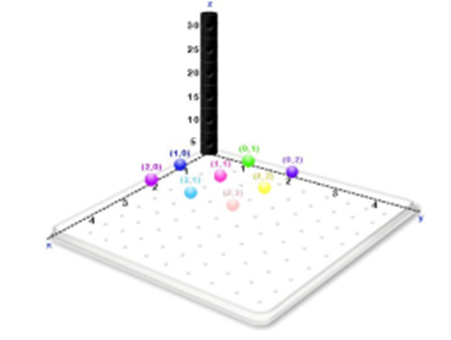
\includegraphics[width=7.5cm, height=7.5cm]{imagenes/NImagen2.png}
    \caption{Representación geométrica}
\end{figure}
\newpage
Entonces podemos elevar cada punto a su valor $z$ apropiado (altura) en 3 dimensiones.\par

\begin{figure}[H]
    \centering
    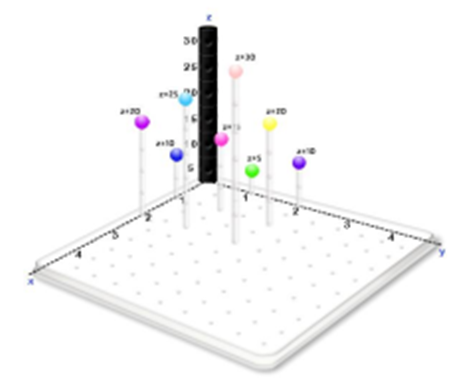
\includegraphics[width=7.5cm, height=7.5cm]{imagenes/Imagen3.png}
    \caption{Con su altura $z$}
\end{figure}

\subsection{Limites y Continuidad}
\section{Limite}
\textbf{Definición:} Sea $D$ un subconjunto de $\mathbb{R}^{n}$ y $f: D \rightarrow \mathbb{R}$, una función definida en $D$, y sea $a$ en un punto de acumulación de $D$. Decimos que el límite de una función $f$ cuando $x$ se acerca a $a$ es $L \in \mathbb{R}$, y lo escribiremos $\lim _{x \rightarrow a} f(x)=L$ si para cada $\epsilon>0$ hay un $\delta>0$ tal que $|f(x)-L|<\epsilon$ si $x \in D$ y $0<d(x, a)<\delta$.\par
Ademas se puede considerar las siguientes propiedades:\par
\begin{enumerate}
    \item Ley constante:\par
          $$
              \lim _{(x, y) \rightarrow(a, b)} c=c
          $$
    \item Leyes de identidad:\par
          $$
              \begin{aligned}
                   & \lim _{(x, y) \rightarrow(a, b)} x=a \\
                   & \lim _{(x, y) \rightarrow(a, b)} y=b
              \end{aligned}
          $$
    \item Ley de la suma:\par
          $$
              \lim _{(x, y) \rightarrow(a, b)}(f(x, y)+g(x, y))=L+M
          $$
    \item Ley de diferencia:\par
          $$
              \lim _{(x, y) \rightarrow(a, b)}(f(x, y)-g(x, y))=L-M
          $$
    \item Ley del múltiplo constante:\par
          $$
              \lim _{(x, y) \rightarrow(a, b)}(c f(x, y))=c L
          $$
    \item Ley del producto:\par
          $$
              \lim _{(x, y) \rightarrow(a, b)}(f(x, y) g(x, y))=L M
          $$
    \item Ley del cociente:\par
          $$
              \lim _{(x, y) \rightarrow(a, b)} \frac{f(x, y)}{g(x, y)}=\frac{L}{M} \text { para } M \neq 0
          $$
    \item Ley de potencia:\par
          $$
              \lim _{(x, y) \rightarrow(a, b)}(f(x, y))^{n}=L^{n}
          $$
          para cualquier entero positivo $n$.\par
    \item Ley de la raíz:
          $$
              \lim _{(x, y) \rightarrow(a, b)} \sqrt[n]{f(x, y)}=\sqrt[n]{L}
          $$
          para todo $L$ si $n$ es impar y positivo, y para $L \geq 0$ si $n$ es par y positivo.\par
\end{enumerate}
\section{Continuidad:}
\textbf{Definición:} Una función $f(x, y)$ es continua en un punto $(a, b)$ de su dominio si se cumplen las siguientes condiciones:
1. $f(a, b)$ existe.\par
2. $\lim _{(x, y) \rightarrow(a, b)} f(x, y)$ existe.\par
3. $\lim _{(x, y) \rightarrow(a, b)} f(x, y)=f(a, b)$.\par
\par
Intuitivamente podemos decir que una función continua de dos variables no tiene saltos.Consideremos el siguiente ejemplo para analizar la continuidad.\par
\textbf{Ejemplo:}\par
Consideramos la función:
$$
    f(x, y)= \begin{cases}\frac{x y^{2}}{x^{2}+y^{4}} & \text { si } x \neq 0 \\ 0 & \text { si } x=0\end{cases}
$$
Queremos comprobar que $f$ no es continua en el punto $(0,0)$. Para conseguirlo veremos que si nos acercamos a $(0,0)$ siguiendo trayectorias diferentes, obtenemos resultados también diferentes. Empezamos por las trayectorias más sencillas: las rectas. Una recta que pase por $(0,0)$ tiene la ecuación:
$$
    a x+b y=0,
$$
donde $a$ y $b$ son números fijos. A continuación estudiaremos dos casos diferentes:
a) Si $b=0$, entonces la recta es $x=0$, es decir, estamos observando la función a lo largo del eje $Y$. En este caso, tenemos que $f(0, y)=0$ para todo $y$, que es una función continua (al ser constante).
b) Si $b \neq 0$, tenemos que $y=-\frac{a}{b} x$. Definimos $c=-\frac{a}{b}$ tal que $y=c x$. El valor que toma la función en este punto es:
$$
    f(x, c x)= \begin{cases}\frac{c^{2} x^{3}}{x^{2}+c^{4} x^{4}} & \text { si } x \neq 0 \\ 0 & \text { si } x=0\end{cases}
$$
$$
    f(x, c x)= \begin{cases}\frac{c^{2} x^{3}}{x^{2}+c^{4} x^{4}} & \text { si } x \neq 0 \\ 0 & \text { si } x=0\end{cases}
$$
Esta función de una variable es continua para todo $c$ fijado, puesto que:
$$
    \lim _{x \rightarrow 0} f(x, c x)=c^{2} \lim _{x \rightarrow 0} \frac{x}{1+c^{4} x^{2}}=0 .
$$
Hemos visto que si nos acercamos a $(0,0)$ siguiendo trayectorias rectas, $f(x, y)$ es continua.
Por otro lado, para comprobar que $f$ no es continua en $(0,0)$, consideramos la trayectoria (parabólica) establecida por $x=y^{2}$. En este caso, la función de una variable que resulta es:
$$
    f\left(y^{2}, y\right)= \begin{cases}\frac{y^{4}}{y^{4}+y^{4}} & \text { si } y \neq 0 \\ 0 & \text { si } y=0\end{cases}
$$
es decir:
$$
    f\left(y^{2}, y\right)= \begin{cases}\frac{1}{2} & \text { si } y \neq 0 \\ 0 & \text { si } y=0\end{cases}
$$
que corresponde claramente a una función discontinua cuando $y=0$, lo cual implica, en particular, que la función $f(x, y)$ no puede ser continua en el punto $(0,0)$.
\printbibliography[heading=bibintoc,
title={Bibliografía}]
\end{document}
